\documentclass[thesis.tex]{subfiles}
\begin{document}
\chapter{Related Work}
\label{chap:related-work}

\section{Android and Mobile OSs}\label{android}
\todo{PUT IN THE DIFFERENCES BETWEEN THE SYSTEMS EXPRESSED IN APPPAL HERE AND MOVE IT TO CH4 WHEN DAVID TELLS YOU TO}

Android is a mobile operating system developed, primarily, by Google. It is by
far the most popular mobile operating system in use being installed on around
83\% of all mobile
handsets\footnote{\url{http://www.idc.com/prodserv/smartphone-os-market-share.jsp}}
with Apple's iOS being its only major competitor (Windows Phone, Blackberry OS
and other mobile operating systems account for only 3\% of the marketshare in
2015).

Despite the dominance of Android its ecosystem is rather fragmented. As shown in
Figure \url{fig:android-versions}, in June 2016 only 10\% of devices used the
latest version of Android, with around 5\% of devices still using a version
released five years prior. The range of different Android versions is often
blamed on the device manufacturers being unwilling to update their devices.
Since the core of Android is open source this has lead to third parties (such as the now-depreciated
CyanogenMod\footnote{\url{http://www.cyanogenmod.org}} and LineageOS~\cite{lineageos_lineageos_2017}) have started developed
custom firmware for Android devices to allow older devices to be upgraded
independently of their manufacturers.

\begin{figure*}
\centering
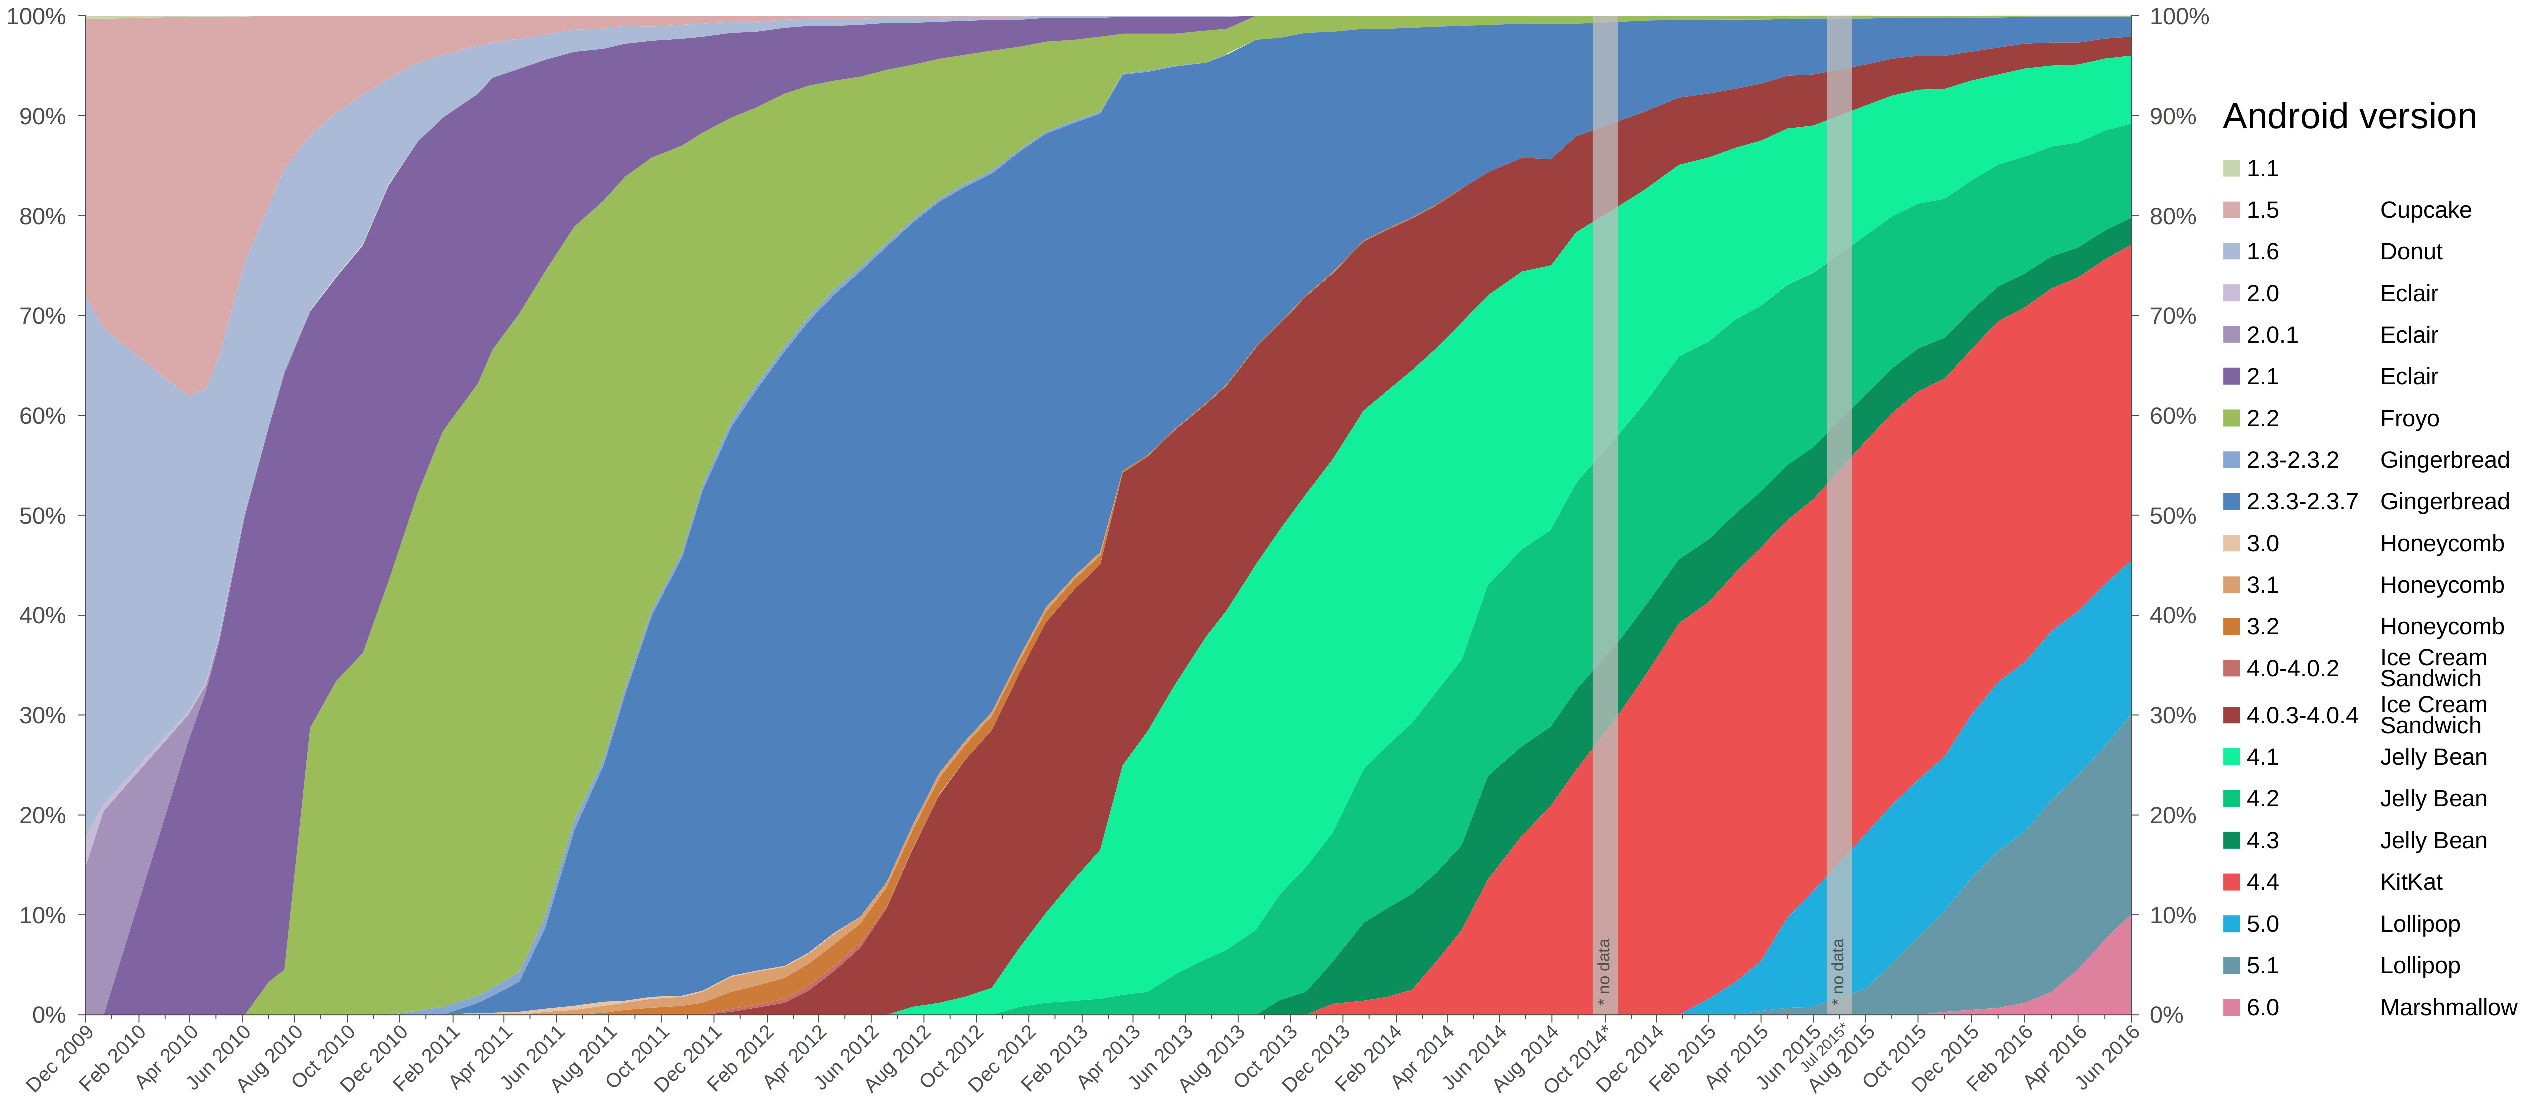
\includegraphics[width=\linewidth]{figures/android-versions.pdf}
\caption[Historical Android version's distribution.]{Historical Android
  version's distribution~\cite{erikrespo_android_2017}.}
\end{figure*}

When building an Android device the manufacturers are also able to make
modifications to the Android firmware. This can be done to support any custom
hardware their device may have, add any additional software or apps, or provide
a custom look or theme to atheir device. Again this creates more variety in the
ecosystem, with few guarantees that any two devices may contain similar features
or hardware. In fact since the core of the Android is the Linux kernel (albeit
without the Linux Standard Base\footnote{The \emph{Linux Standard Base} is a
  specification produced by the Linux foundation that describes what a stardard
  Linux system should contain and how it should be organised. Android uses its own
  system which differs most noticably by the different filesystem structures and
  the use of user IDs to separate apps rather than users~\cite{linux_foundation_lsb_2015}.}, and with additional
patches) it can be ported to other architectures (such as X86 and MIPS), and
used in other devices (such as set-top boxes and TVs, watches, and cars) with
relative ease.

To give developers a somewhat stable base to develop for Google developed the
\ac{CTS}\footnote{\url{https://source.android.com/compatibility/cts/index.html}},
and \ac{CDD}\footnote{\url{https://source.android.com/compatibility/android-cdd.html}}.
The \ac{CTS} is a series of unit tests that check basic Android functionality and
behavior. The \ac{CDD} is a document that describes what hardware an Android device
should have and how the device and it's software should be built. If a device
manufacturer wishes their device to run Google's Play Store (the largest Android
app marketplace), then they are required to show they can pass the \ac{CTS} and are
in compliance with the \ac{CDD}.

\section{Authorization Logic and Fine Grained Permission Systems}
\label{sec:authorization-logic}

Our work on AppPAL extends Becker's work on SecPAL to support the
policies surrounding the mobile ecosystem.  This work is, of course,
not done in isolation but part of a larger work into policy languages.
In this section we review some of the many policy languages AppPAL
grew from and was inspired by, as well as the fine-grained permission
schemes that have become an important mechanism for enforcing policies
on Android devices and have added to work on policy languages
themselves.


\subsection{Policy Languages}
%\subsection{PolicyMaker}

PolicyMaker~\cite{blaze_decentralized_1996} was created to give a
language for permitted actions.  It grew out of the logics of
authentication of Wobber, Abadi, Burrows and Lampson~\cite{wobber_authentication_1994,abadi_calculus_1991}; as well as a
dissatisfaction with identification mechanisms.  X.509 and PGP
certificates had given a mechanism for identifying users; at the time
however, they did not give any means to link the users to what users
were allowed to do.

To describe the authorizations trust information is contained within
assertions.  A collection of assertions form the policy.  An assertion
has a source (either the local policy document or a public key). The
source \emph{asserts} that a key (or more complex arrangements such as
three of four keys) is permitted to perform any action that matches
the \emph{filter}.  The filter itself is essentially an arbitrary
program that can decide if an action is permitted.
Blaze~\etal~provide examples using regular expressions and a reduced
version of AWK~\cite{aho_awk-pattern_1979} they call \emph{AWKWARD},
though they note that any programming language could be used.  The
collection of these authorizations on a machine forms the policy for
the device which can be queried by a PolicyMaker key \emph{requesting}
a given action.

Blaze~\etal~give an example of this scheme being used as part of an
email server.  A user, Alice, identified by key \texttt{0x12345678} is
permitted to send emails with the from header set to Alice and the
organisation set to Bob Labs.

A PolicyMaker instance is installed on a server and allowed to receive queries and give answers.
The policy is installed on the server as follows:

\begin{lstlisting}
policy ASSERTS
  pgp:'0x12345678'
  WHERE PREDICATE=regexp:'(From: Alice) &&
    (Organization: Bob Labs)';
\end{lstlisting}

When Alice tries to send an email using a PolicyMaker enhanced SMTP
client she signs and sends her message using her key.  The mailserver
checks the signature and queries the policy server with her message:

\begin{lstlisting}
  pgp:'0x12345678'
  REQUESTS  'From: Alice
             Organization: Bob Labs

             Hello World!';
\end{lstlisting}

If Alice's request is accepted then the SMTP server will send the
message.  If it doesn't match the policy then it won't.

PolicyMaker was used as the basis for the KeyNote Trust Management
System~\cite{blaze_role_1999,blaze_keynote:_1998} which simplified the
filter languages from any arbitrary language to a purpose built one
based on C that always returned a boolean answer, allowed the policy
server to do the signature verification instead of the querying
application, and tweaked the syntax for readability.  It was designed
to trade some of the generality of PolicyMaker for a more realistic
scenario using public-key infrastructure.  The equivalent policy for KeyNote could be written:

\begin{lstlisting}
Authorizer: "POLICY"
Licensees: "RSA:abc123"

KeyNote-Version: "2"
Local-Constants: Alice="RSA:12345678" 
Authorizer: "RSA:abc123"
Conditions: (app_domain == "RFC822-EMAIL") &&
    (name="Alice") &&
    (organization="Bob Labs");
\end{lstlisting}

Checking whether a PolicyMaker or KeyNote policy is satisfied is
NP-hard~\cite{blaze_compliance_1998}.  It is not tractable as checking
PolicyMaker assertions can involve arbitrary programs written in
Turing complete languages.  Deciding whether a program will stop when
given an arbitrary input is analogous to the halting problem.  So in
general it is not known whether a PolicyMaker program which takes an
arbitrary request and an unconstrained set of checking functions will
terminate: it is undecidable.  Blaze~\etal{} give
some restrictions that guarantee polynomial time checking: a function
must be authentic (not fake another functions result), monotonic, and
run in polynomial time for all inputs pertinent to a request.  This
reduced the expressiveness however.

Another weakness of these languages is that they cannot express
general relationships as the subjects of the policy cannot be a
variable.  You cannot have, for example, a policy where the subject is
a set of users.  The example policy could not be written as
\emph{anyone working in R\&D can send email from Bob Labs.}  This
restriction made the languages less expressive than they might
otherwise have been.

%\subsection{SPKI/SDSI}

In contrast to PolicyMaker SPKI/SDSI~\cite{ellison_spki_1999} is
designed to associate keys with roles.  A user, Alice with key~$K_A$,
can present a certificate that says she can act as a \emph{Bob Labs
employee} (authorized by Bob with key~$K_B$) for one~year.

\begin{equation*}
  (K_A,~\text{\tt BobLabsEmployee},~K_B,~1~\text{year})
\end{equation*}

Bob can also create authorization certificates to permit his employees
to send emails, and can optionally delegate the decision further.

\begin{equation*}
 (K_B,~(K_B,~\text{\tt BobLabsEmployee}),~\bot,~\text{\ttfamily send\_email},~1~\text{year})
\end{equation*}

Where PolicyMaker let an administrator check if a specific action was
permitted by a specific user, SPKI/SDSI lets administrators associate
users with roles and roles with tasks.  The SPKI/SDSI version of the
email sending policy doesn't specify that all emails sent by Employees
must have a field listing the lab as the sending organization; that
part of the policy must be implemented by whatever implemented the
\texttt{send\_email} functionality.  One of the large advantages of
SPKI/SDSI is that it allows a higher-level view of the policy by
associating groups of users with a role, and roles with allowed
actions.

A weakness of SPKI/SDSI however was that the language was not designed
with formal semantics.  This meant that it was not possible to define
precisely what promises the language gave or how to extend it safely
or even exactly what it does.  All these things must be inferred from
RFC 2693 which loosely defined it~\cite{ellison_spki_1999}. There were
several later attempts to fit a semantics to the
language~\cite{joseph_y._halpern_logic_1999,abadi_sdsis_1998,howell_formal_2000},
however not all covered every aspect of SPKI/SDSIs features.

The focus on roles leads to the RT family of
languages~\cite{ninghui_li_design_2002}, which associates policy
decisions with roles similar to how \ac{RBAC} systems associate access
decisions to the roles a user holds.  Policies are expressed as Horn
clauses.  A rule such as:

\begin{lstlisting}[language=prolog]
Bob.employee :- alice.
Bob.employee.sendEmail :- Bob.employee.
\end{lstlisting}

Should be read as \emph{Bob says Alice is an employee.  Bob says an
employee can send emails if they are an employee.}  Li~\etal{}
describe many different variants of RT each with increasing numbers of
features.  The most basic variant is
\RT{0}{}~\cite{li_distributed_2003}, but \RT{1}{} adds support for
parameterized roles, and \RT{2}{} adds logical objects on top of the
roles.  As well as these variants, the RT family of languages have
support for optional feature sets: \RT{}{T} allows for policies with
thresholds (i.e. Alice can send an email if two out of three of the
board members approve it), \RT{}{C} adds constraints, and \RT{}{D}
adds delegation~\cite{ninghui_li_design_2002}.

Unlike PolicyMaker, the RT family of languages is tractable, they can
guarantee that a query will be answered soundly in polynomial time
with respect to the size of the policy.  To give this guarantee trust
languages some trust languages such as
Binder~\cite{detreville_binder_2002} and
Delegation~Logic~\cite{li_delegation_2003,li_practically_2000} had
shown that they could be reduced to Datalog, a database language with
known complexity guarantees and fast evaluation based on Prolog.  One
limitation of Datalog is that it cannot describe structured data: for
example consider an administrator who wishes to write a policy rule
that says Alice can send email between 9am and 5pm.  We can imagine in
the policy rule having some function to fetch the time and another to
compare whether it is within that range.  In Datalog we cannot
trivially write this function and instead have to enumerate each
possible time in that domain and state whether it is within that
period. For example:

\begin{lstlisting}
  between_9_to_5(9:00).
  between_9_to_5(9:01).
  between_9_to_5(9:02).
  ...
  between_9_to_5(16:59).
  between_9_to_5(17:00).
\end{lstlisting}

This is obviously undesirable: we would need to add almost 500
statements to the knowledge base for resolution of the time to
minutes, and tens of thousands if we need the time accurate to
seconds.  More generally whenever there is data that has structure
such as file paths, times or numeric intervals; Datalog databases can
become large and start to become intractable.

To solve this problem Li~\etal{}~proposed a modified version of
Datalog called Datalog\textsuperscript{C}~\cite{li_datalog_2003},
based on Constraint
Datalog~\cite{revesz_constraint_1995,revesz_safe_1998}, that better
supported constraints and kept Datalog's tractability, with a focus on
the constraints typical to a policy languages instead of those for
database programming.

Datalog\textsuperscript{C} has also been used as a foundation for many
other policy languages including SecPAL based
languages~\cite{aziz_secpal4dsa:_2011,becker_secpal:_2010,becker_framework_2009,hallett_apppal_2016}
and DKAL~\cite{gurevich_dkal:_2008}, as well as
Cassandra~\cite{becker_cassandra:_2004}.

Cassandra is a trust management language designed to model large
systems, in particular the NHS Spine: a system designed to enable
healthcare workers to share patient data.  Cassandra is role-based but
rather than having principals hold or be given roles, principals
\emph{activate} roles when they need to act in that capacity.  This
allows a single principal to hold different roles with different
access capabilities at different times. \todo{More
explanation... summarise from Becker's thesis.  Give an example.}

\todo{DKAL}

\subsubsection{XACML}

XACML is a standardised policy language~\cite{oasis_extensible_2013}
that can be extended to fit many scenarios. It is an attribute based
policy language, but can also describe role-based policies; and has
industrial support from \emph{Oracle}.  It is worthy of special
attention as it has become an extremely popular policy language from
both an industrial and academic standpoint.  As such it is important
to summarize and briefly describe why we chose to base our own work on
SecPAL, a comparatively obscure policy language, instead of the more
popular XACML.

XACML policies are expressed as sets of \emph{rules} that describe
whether a specific action should be allowed or denied. When making a
\emph{request} if a rule's target matches the request then the
appropriate action should be taken. Rules are combined into policies
and may contain many rules which can contradict each other if multiple
ones match a given request. To handle contraditions between rules a
\emph{combining algorithm} may be used to decide how to
proceed. Typical algorithms include:

\begin{description}
  \item[Permit-overrides] where if a single rule gives a permit result then the request is permitted.
  \item[Deny-overrides] where if a single rule gives a deny result then then the request is denied.
  \item[First-applicable] where the rules are given an order of precedence and the first rule in the order that gives a result decides the outcome.
  \item[Only-one-applicable] where only one rule may match, and if there are multiple matches an error is returned.
\end{description}

XACML is a powerful access control and policy language with a published
standard~\cite{oasis_extensible_2013}. It is generic and is used in industry as
a policy language for access control decisions, and there are tools available to
help policy authors write policies in it. Whilst XACML might seem like a
suitable language to model mobile ecosystems, it suffers from various issues.

Readability was a design goal for SecPAL. Its notation is similar to natural
language. Alternate notations based on XML do exist (Becker hints at them in the
SecPAL technical report~\cite{becker_secpal:_2010}); though these are to aid
computerised parsing of SecPAL not human legibility. In contrast, XACML's
default syntax is difficult to read. XACML policies are verbose, and written in
XML. To help developers write policies alternative notations are available that
compile into XACML's XML notation. ALFA is an alternate notation for
XACML~\cite{oasis_xacml_technical_comitee_abbreviated_2015}. The XACML
developers maintain ALFA, however others notations exist including graphical
languages~\cite{henrik_nergaard_scratch-based_2015}, languages based on
propositional logic~\cite{zhang_synthesising_2004} and answer set
programming~\cite{ramli_xacml_2012}.

\todo{MORE DETAIL EMPHASISE SEMANTIC PROBLEMS}
XACML does not have well-defined semantics. XACML's designers used natural
language to describe the semantics of XACML. This has made the semantics
notoriously difficult to interpret~\cite{ramli_detecting_2015}. There have been
several attempts to describe XACML's semantics
formally~\cite{ramli_xacml_2012,ramli_logic_2014,bryans_reasoning_2005}. These
help specify XACML but the lack of a single standard semantics make it less
attractive to extend to a new domain. In contrast, SecPAL's semantics are given
precisely by Becker~\cite{becker_secpal:_2010}

Whilst XACML 3.0 does support delegation~\cite{oasis_xacml_2010}, earlier
versions do not. The XACML 3.0 standard was published in 2013, after deciding to
start work with SecPAL.

\todo{GIVE EXAMPLES OF XACMLS SYNTAX}

\subsection{Fine Grained Permission Systems}
\subsubsection{Dr.~Android and Mr.~Hide}
\subsubsection{Aurasium}
\subsubsection{CRePE}
\subsubsection{Kirin}
\subsubsection{SEAndroid}

\section{Static analysis tools}

There have been many static tools developed that can infer complex
properties about
apps~\cite{felt_android_2011,song_integrated_2016,antonin_carette_investigating_2017,schmidt_static_2009,enck_taintdroid:_2014}.
Leveraging these tools in a policy language lets us make statements about the
properties they can infer, without having to reimplement the functionality.
Despite the power of these tools it is not obvious how they should integrate
with the policies surrounding the mobile ecosystem. Running and configuring each
It isn't clear when each tool should run, or how to configure them to enforce a
policy rule. By incorporating these tools into a policy language, such as
SecPAL, we can act as a glue-layer between the policies of the mobile ecosystem
and the research into the properties of code.

\section{Datalog}
\label{ssec:datalog}

\todo{lift the citations from the 1yr}

Datalog is used in the implementation of several authorization
logics~\cite{detreville_binder_2002,li_distributed_2003,becker_secpal:_2010}. A brief explanation of the languageand its variants is given for some context as to how these languages
can be implemented and the limitations the languages inherit from
Datalog.

Datalog is a database language. It was created from a simplification
of general logic programming. The language is based on first order
logic; evaluation of Datalog is both sound and complete (under the
\ac{CWA}). Datalog is used as the basis for several of the
authorization logics including SecPAL. We will review several
evaluation strategies used for querying Datalog knowledge bases as
most common method (bottom-up) is not particularly suitable for
authorization logic application

Datalog programs are presented as series of Horn clauses in the same
way as Prolog. There are additional restrictions, however: all
variables in the head of a clause must be present in the body, and no
parameter can be a nested predicate.  Datalog programs are split into
two sets. The \ac{EDB} has all ground (containing no free variables)
facts. The \ac{IDB} contains rules for deriving more facts.

\subsection{Evaluation Strategies}

The bottom-up or Gauss-Seidel method is a simple evaluation strategy~\cite{???}. Given a
Datalog program we try every constant with every rule from the IDB. When a rule is
found to be true we add it to the set of facts. Repeat until a fixed point (or the required fact) is known. If a queried fact is still unknown when the search terminates then it is
false; as Datalog assumes the CWA. The strategy is complete and will always terminate.
Querying the database is fast once all facts have been inferred and large joins are quick.
This strategy ends up computing all known facts. It is less useful when only a subset are
interesting. The magic sets~\cite{???} rewriting rule avoids this problem. Interesting constants
are marked as magic. The knowledge base is a graph: nodes related to a magic one are
also magic. Rules in the IDB are rewritten to check constants used in the inference are
also be magic. This cuts down on irrelevant results: anything that isn't interesting will
not be in the magic set.

The SLD-resolution algorithm works top down. It starts with a goal and
then constructs a proof tree. Transitions are applications of rules
from the IDB. Nodes are either facts (the leaves) or further
branches. If there is a subtree from the query node to true facts then
it is true. Prolog uses this strategy. Its memory efficient as it
searches the tree in a depth-first manner. Breadth-first and other
tree traversal searches are also possible as are parallel
strategies. The top-down strategy is less commonly used with Datalog
programs. Saving previous search results (called tabling) is often
used with this strategy to speed queries.

The SLD resolution may not terminate if there are a set of rules that
set up an infinite loop (for instance the rule \lstinline!a(X) :- a(X).!).
Because Prolog has an infinite number of constants (integers
for example) it is also possible to construct queries which return an
infinite number of answers. Datalog does not suffer from this as it's
programs must contain all known constants because of the \ac{CWA} (and
therefore there are a finite number of them).


\subsection{Datalog Variants}

Datalog does not support negation. It is not possible to write
rules which depend on false facts.  This is inconvenient as it is
natural to write rules which rely upon a negative result: for example
an app is safe to run if it is not malware.  Whilst this extension to Datalog is
not strictly required (the \ac{CWA} can be used) it makes programs clearer.

A version of Datalog with negation called
\emph{Datalog$^\lnot$}~\cite{Ceri:1989ff} is made by allowing negation in clause
bodies. Two sets of known facts are defined: those that are true and those that
are false.  When deciding if a fact is satisfied by a Datalog program if the
fact is not negated then it must be inferable by the rules of the program; if
the fact is negated then it must not be satisfiable.  

In unmodified Datalog if the bottom-up strategy
is used all possible facts are inferred. These facts form a single, minimal
model of the Datalog program.  In Datalog$^\lnot$ the program \textsf{safe(game)
:- $\mathsf\lnot$ malware(game).} has two minimal models that are inconsistent
with each other: \code{safe(game)} and \code{malware(game)}.  This can make
analysis problematic as the \ac{CWA} is broken. A further variant called
\emph{Stratified Datalog$^\lnot$} avoids this by further restricting what can be
negated and defining an evaluation order~\cite{Apt:1986vj}.

Constraint Datalog (Datalog$^C$~\cite{Li:2003ix}) is based
on constraint logic programming.  Constraint logic programming allows
relationships to be defined with general relationships (ordering by time
for example)\footnote{Full logic programming languages like Prolog often
support these relations. Datalog, however, does not as it would require all
possible times to be named, and described in order to each other.} rather than with just the pre-defined predicates.  Being able to
define relations in terms of general relations is convenient for
authorization logics as it lets things be defined in terms of time or
other general (and infinite) concepts. 
Expressing these relations in Datalog is hard, as described earlier.

While some constraints applied to domains are tractable (such as
trees, ordering and discrete domains) Li~\etal{}~could not show
all were.  Policy languages that use constraint Datalog often apply
additional restrictions on how constraints can be used.  Variable independence
conditions~\cite{Chomicki:2000tz} have been suggested as a \emph{middle-ground}
as they can simplify the query evaluation while still keeping the extra
expressiveness Datalog with constraints allows.

\todo{Add a bit on probabilistic datalog by N Fuhr!}

\end{document}

%%% Local Variables:
%%% mode: latex
%%% TeX-master: "../ch7.tex"
%%% End:
